\section{Screen Layout Model}
In the early 70s, Xerox PARC in California launched the Smalltalk project with the goal of
conceiving and developing new more natural ways to communicate with PCs \cite{Goldberg}.
Perhaps the most conspicuous among several significant achievements of this endeavor is the
idea of applying the desktop metaphor to the display screen. This metaphor comprises a desktop
and the collection of possibly mutually overlapping pages of paper laid out on it. By projecting
such a configuration onto the screen surface we get the familiar picture of Fig \ref{fig:desktop}
showing a collection of partially or totally visible rectangular areas on a background,
so-called \emph{windows} or \emph{viewers}.
\begin{figure}[h!]
  \centering
  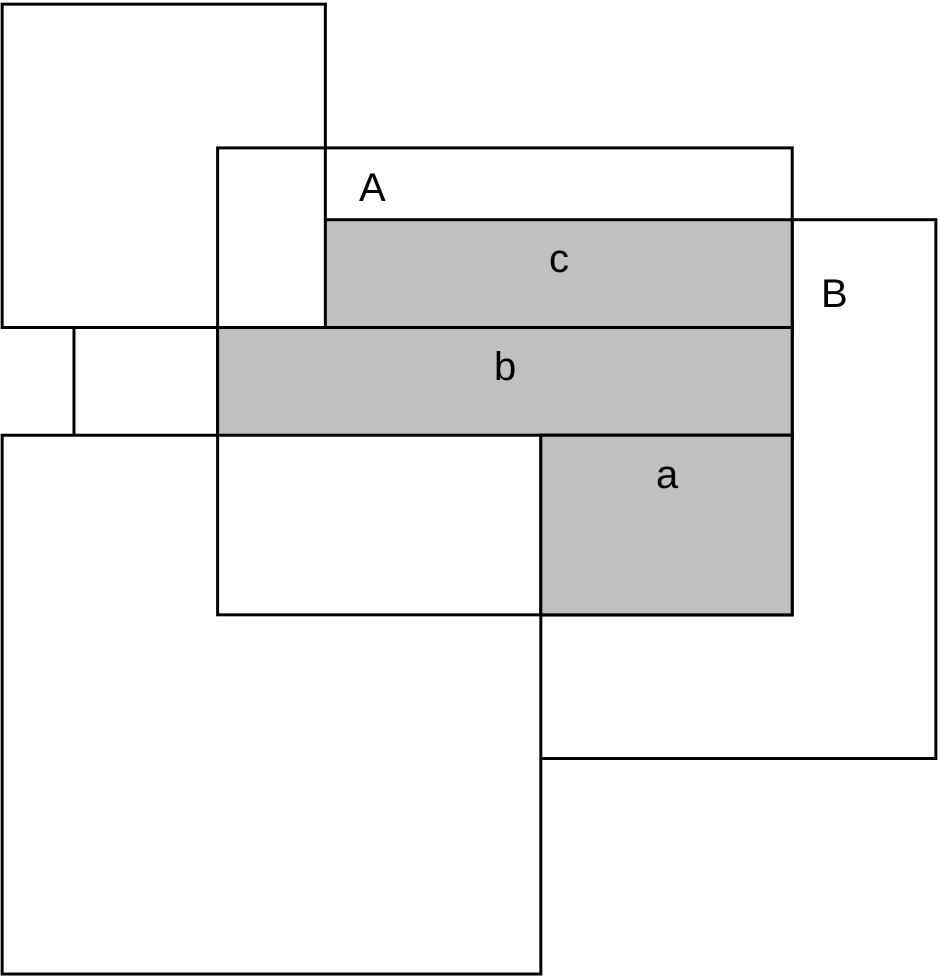
\includegraphics[width=.6\textwidth]{i/4}
  \caption{Desktop showing partially overlapping viewers}
  \label{fig:desktop}
\end{figure}

The desktop metaphor is used by many modern OSes and user interface shells both as
\begin{table}[h!]
  \centering
  \begin{tabular}{c c l}
    a       & for    & to \\\hline
    natural & the    & separate displayed data \\
    model   & system & belonging to different tasks, and \\\hline
    power   &        & organize the display screen \\
    -ful    & users  & interactively, according to \\
    tool    &        & individual taste and preference.
  \end{tabular}
\end{table}

However, in this metaphor there are inherent drawbacks, primarily connected with overlapping.
\begin{itemize}
  \item[$1^{st}$,] any efficient management of overlapping viewers must rely on
    \begin{itemize}
      \item[-] a subordinate management of (arbitrary) sub-rectangles, and
      \item[-] sophisticated clipping operations.
    \end{itemize}
    This is so because partially overlapped viewers must be partially restored under control
    of the \emph{viewer manager}. For example, in Fig \ref{fig:desktop}, rectangles $a$, $b$,
    and $c$ in viewer $B$ ought to be restored individually after closing of $A$.
  \item[$2^{nd}$,] there is a significant danger of covering viewers completely and losing them forever.
  \item[$3^{rd}$,] no canonical heuristic algorithms exist for automatic allocation
    of screen space to newly opened viewers.
\end{itemize}

Experience has shown that partial overlapping is desirable and beneficial in rare cases only,
so the additional complexity of its management is hard to justify. \cite{Binding, Wille}
Therefore, alternate strategies to structure a display screen have been looked for.
An interesting class of established solutions can be titled as \emph{tiling}.
There are at least 2 variants. \cite{Cohen}

Perhaps the most \emph{unconstrained} (hence obvious) one is based on iterated horizontal
or vertical splitting of existing viewers. Starting with the full screen and successively
opening $A$, $B$, $C$, $D$, $E$, and $F$ we get to a configuration as in Fig \ref{fig:tiling}.
\begin{figure}[h!]
  \centering
  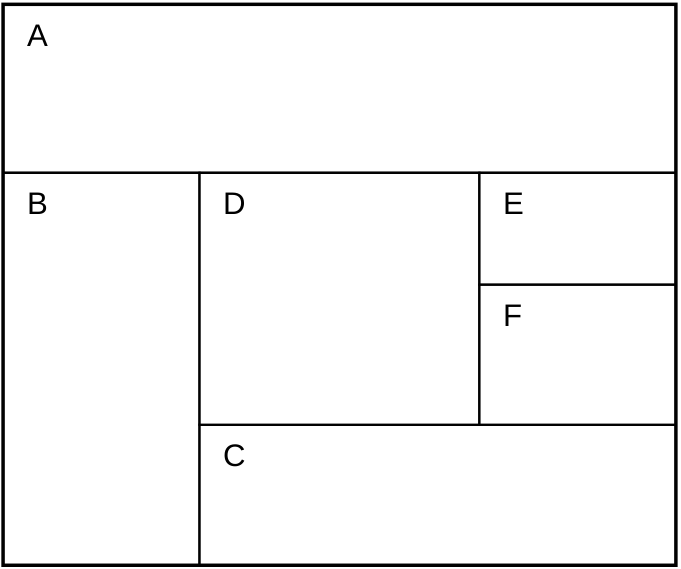
\includegraphics[width=.6\textwidth]{i/5}
  \caption{Viewer configuration resulting from unconstrained tiling}
  \label{fig:tiling}
\end{figure}

The $2^{nd}$ variant is \emph{hierarchic tiling}. Again, the hierarchy starts with a full screen
that is now decomposed into a number of \emph{vertical tracks}, each of which is further
decomposed into a number of horizontal viewers. We decided in favor of this kind of tiling
in Oberon, mainly because the algorithm of reusing the area of a closed viewer is simpler
and more uniform. For example, assume that in Fig \ref{fig:tiling} viewer $F$ has been closed.
Then, it is straightforward to reverse the previous opening operation by extending viewer $E$
at its bottom end. However, if the closed viewer is $B$, no such simple procedure exists.
For example, the freed area can be shared between viewers $C$ and $D$ by making them extend
to their left. Clearly, no such complicated situations can occur in the case of hierarchic tiling.

It is also used in Xerox PARC's Cedar system \cite{Teitelman}. However, Oberon differs in:
\begin{itemize}
  \item[$1^{st}$,] It supports quick temporary context switching by overlaying one track or
    any contiguous sequence of tracks with new layers.  In Fig \ref{fig:overlay} a snapshot
    \begin{figure}[h!]
      \centering
      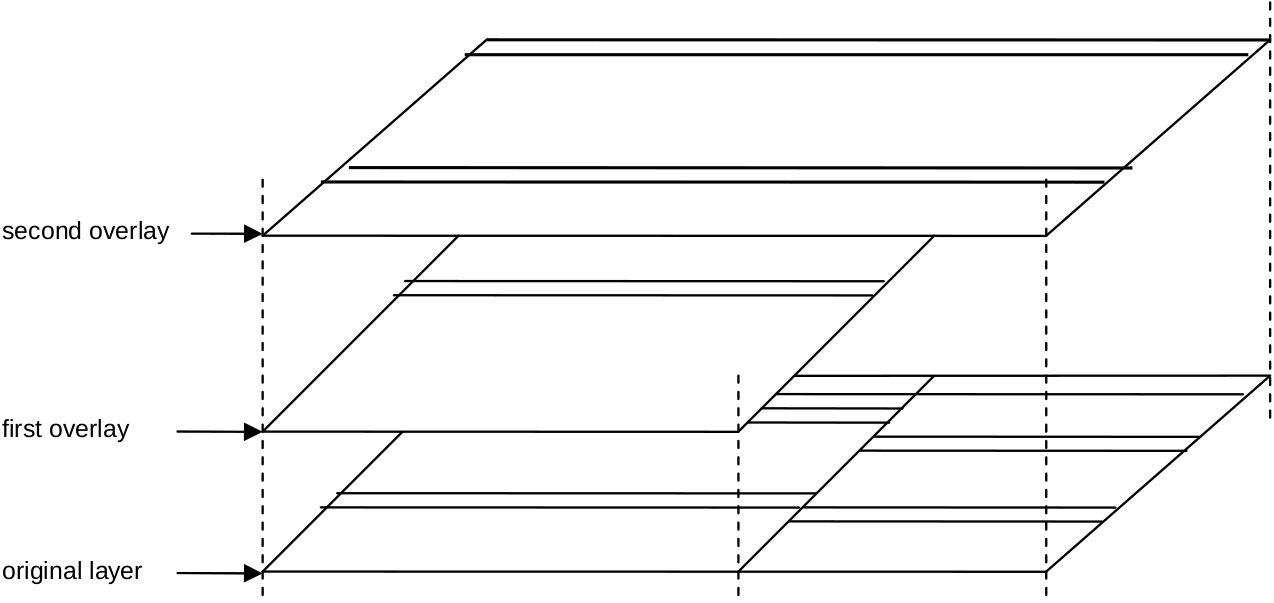
\includegraphics[width=.8\textwidth]{i/6}
      \caption{Overlay of tracks and sequences of tracks}
      \label{fig:overlay}
    \end{figure}
    of a standard display screen is graphically represented. It suggests 2 original tracks
    and 2 levels of overlay, where the top layer is screen-filling.

  \item[$2^{nd}$,] Oberon displays do not provide reserved areas for system-wide facilities, while
    standard Cedar screens feature a command row at the top and an icon row at the bottom. And

  \item[$3^{rd}$,] It is based on a different heuristic strategy for the automatic placement
    of new viewers. As a Cedar default invariant, the area of every track is divided up evenly
    among the viewers in this track. When a new viewer is to be placed, the existing viewers
    in the track are requested to reduce their size and move up appropriately. The newly opened
    is then allocated in the freed spot at the bottom. In contrast, Oberon normally splits
    the largest existing viewer in a given track into 2 halves of equal size. As an advantage
    of this latter allocation strategy we note that existing contents are kept stable.
\end{itemize}
